\subsection{Current Interface and Actual Captures}
Only the selected step runs its widgets. Decision shows the policy result and probabilities. Evidence shows a feature value, maintained definition and selected-class SHAP effect. Risk profile shows capacity, the tolerance total, binding constraint and required confidence. Explanation check shows the candidate, claim report and separately verified output. Each step includes historical date/horizon, confidence and a short interpretation note.
\begin{inlinefigure}\centering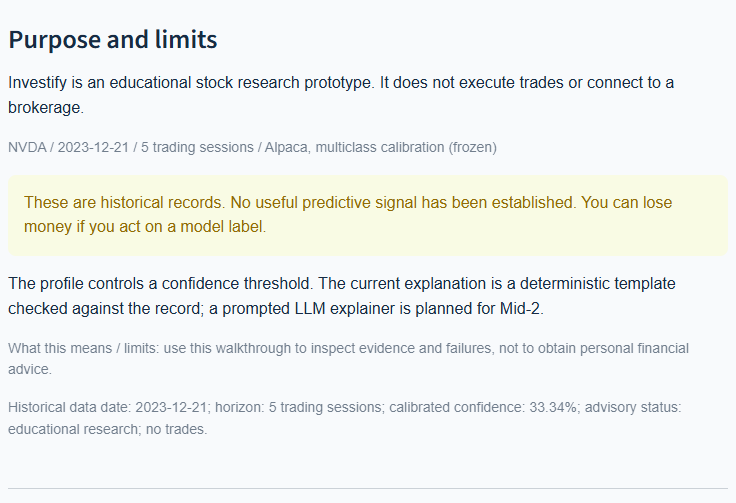
\includegraphics[width=\linewidth]{figures/presenter_browser_20261014_v11_run04/onboarding.png}\caption{Current onboarding purpose, risks, date/horizon and confidence.}\label{fig:browser-onboarding}\end{inlinefigure}
The captures below are actual views from the revised browser journey. They show the current Observe headline, profile threshold and policy-aware fallback; the capture receipt records their source files and image hashes.
\begin{inlinefigure}\centering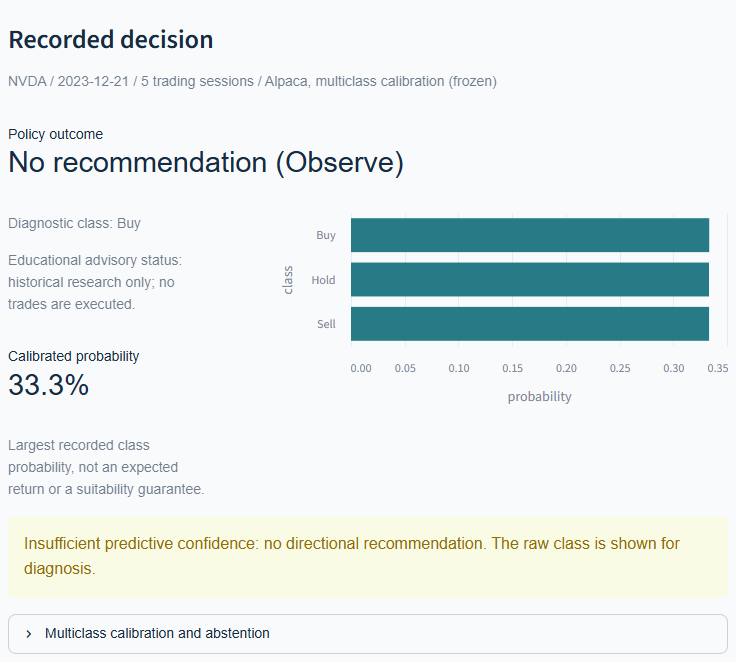
\includegraphics[width=\linewidth]{figures/presenter_browser_20261014_v11_run04/decision.png}\caption{Current decision panel with the full Observe headline and a secondary diagnostic class.}\label{fig:browser-decision}\end{inlinefigure}
\begin{inlinefigure}\centering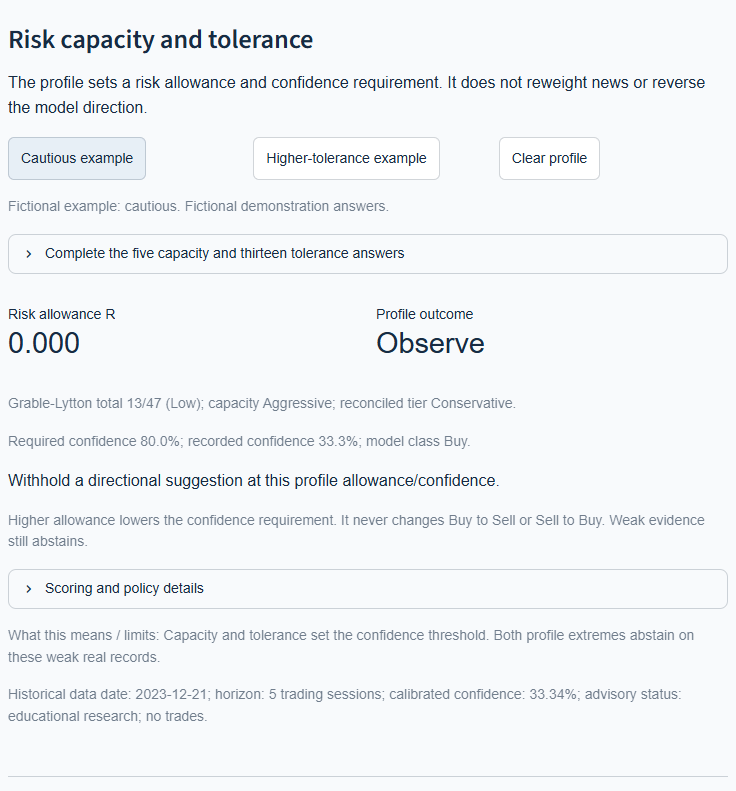
\includegraphics[width=\linewidth]{figures/presenter_browser_20261014_v11_run04/profile.png}\caption{Current cautious profile: tolerance 13/47, allowance zero and 80\% required confidence.}\label{fig:browser-profile}\end{inlinefigure}
\begin{inlinefigure}\centering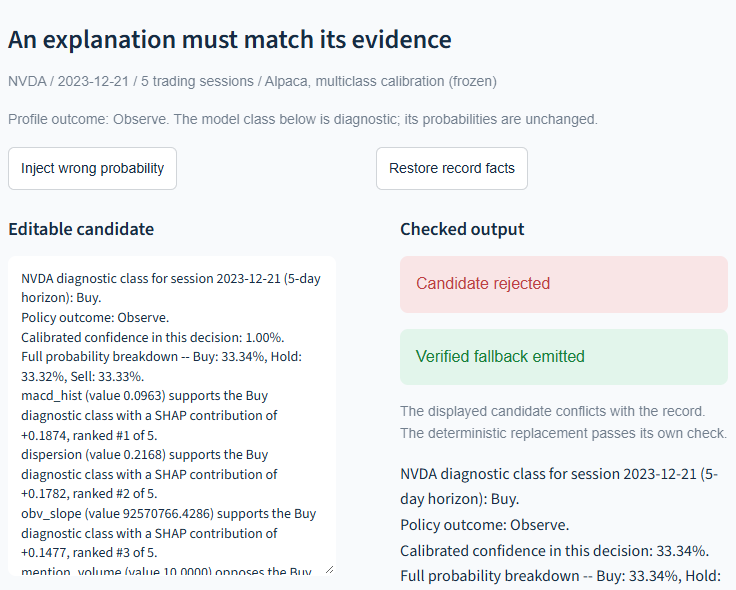
\includegraphics[width=\linewidth]{figures/presenter_browser_20261014_v11_run04/explanation.png}\caption{Current displayed-probability corruption and checked Observe fallback.}\label{fig:browser-fallback}\end{inlinefigure}
